\chapter{引言}\label{chap:introduction}
近几十年来, 弹性波散射问题及其反问题在工程领域和数学领域都得到了广泛研究\cite{landau}.  特别地, 弹性波反散射问题在地球物理领域、石油勘探领域中发展迅速. 
弹性波反散射问题是利用接收到的弹性波散射数据去探寻障碍物的位置、形状、大小.  相比于声波, 弹性波是由横波和纵波耦合而成的矢量波, 因此研究难度更大.  除此之外反问题普遍具有强非线性及高度不适定性, 这导致弹性波反散射问题的研究更具挑战性和吸引力. 目前,在数学领域,学者们主要研究的弹性波反散射问题为全空间背景下的弹性波反散射问题\cite{bonnet2005inverse,bao2018inverse}和粗糙表面的弹性波反散射问题\cite{liu2019near}.  全空间背景下的弹性波反散射问题有反障碍物问题和反源问题; 粗糙表面的弹性波反散射问题又有局部粗糙面和无穷粗糙面两种. 另一方面,在勘探地球物理领域, 弹性波是在地表以下传播的, 这是一个半空间模型. 因此,本文将联系实际,从数学的角度针对半空间弹性波散射问题和反散射问题加以研究,特别是考虑如何从数值上构造一个高效稳定的算法来重构障碍物.  而且,该直接成像法是基于逆时偏移的思想,不需要事先知道障碍物是否可穿透以及其不可穿透时边界条件的先验信息. 
\section{研究背景}
 散射理论研究在二十世纪的数学物理学界占据了非常重要的地位. 通俗地讲, 弹性波的散射问题, 就是研究当入射波(地震源、可控震源)从一种弹性介质进入另一种弹性介质或是碰到障碍物 (散射体) 时产生的效应.  与声波、电磁波散射问题提法类似, 弹性波散射问题只是把控制方程换成了 Navier 方程. 特别地, 如果我们把弹性波总场 $u(x)$ 看作是入射波 $u^i(x)$ 和散射波 $u^s(x)$的和,那么正散射问题就是根据入射波 $u^i(x)$,障碍物的物理特性以及弹性波方程去求解散射波 $u^s(x)$.  本文更感兴趣的反散射问题就是利用散射波$u^s(x)$ 或是 $u^s(x)$ 在无穷远处的渐近形式来重构障碍物的位置、大小、形状. 在研究反散射问题前, 对正散射问题有一个清晰的理解是必不可少的. 因此, 在后文中, 我们先来研究半空间弹性波正散射问题. 
\section{半空间弹性波散射问题介绍}
传统的地震波数据处理常常是基于声波方程的, 这是由于假设地球中只能传播压缩波 (compressional waves),又称 p 波 \cite{yan2008isotropic}.  尽管有了这种假设可以使得实际操作可以减少计算量,且便于理论分析,但是这不利于完整地利用地震波信息.  事实上, 由于地球是一个弹性体,同时存在 p波和 s波, 因此我们可以将地下看成是一个填充弹性介质的半空间. 弹性波的传播主要是用弹性波方程描述的. 在本文中, 我们将重点研究二维半空间时谐弹性波散射问题与反散射问题.  令 x 为半空间中的一个质点, 即 
\ben
x:=(x_1,x_2)^T\in\R^2_+:=\{(y_1,y_2)^T\in\R^2:y_2>0\}.
\een
令 $u(x):=(u_1(x),u_2(x))\in\C^2 $ 为在 x 处的位移.  假设弹性介质是线性各项同性均匀介质, 其 {Lam\'{e}} 常数 $\lambda$ 和 $\mu$ 满足 $\lam>0,\mu>0$, 密度函数为 $\rho$, 角频率为 $\omega>0$, 则位移函数满足如下时谐弹性波方程:
\ben
\nabla\cdot\sigma(u(x)) +\om^2 u(x)= -f(x),
\een
这里 $f(x)$ 是点x 处的外力,应力张量 $\sigma(u)\in \C^{2\times2}$ 是2阶张量, 它与应变张量 $\ep(u)\in \C^{2\times2}$ 一起满足如下本构关系 (胡克定律):
\ben
& &\sigma(u) = 2\mu\ep(u) + \lambda\div u \I \ , \\ 
& & \ep(u)=\frac{1}{2}(\na u +(\na u)^T).
\een
其中 $\I\in\R^{2\times 2}$ 是二阶恒等矩阵,$\nabla u$ 是位移梯度张量,且其每个元素为 
\ben
(\na u)_{ij}=\pa u_i(x)/\pa x_j   .
\een 
为了表述简便, 我们在后文中都假设背景介质的密度为 $\rho=1$. 特别地, $\sigma(u)\nu$ 表示在方向 $\nu$ 上的应力. 为了简便,我们定义弹性波算子 :
\ben
& &\Delta_e u:=(\lambda+\mu)\nabla\div \ u+\mu\Delta u.
\een
易得 $\Delta_e u(x) = \nabla\cdot \sigma(u(x))$. 
于是, 弹性波 u(x) 满足如下弹性波方程: 
\be
& &\Delta_e u(x)+ \rho\,\omega^2u(x)= -f(x) .
\ee
除此之外弹性波在地表满足自由表面边界条件 \cite{ela_reverse,grant1965interpretation} 即法向应力为零. 有了如上表述,我们就可以提出如下半空间弹性波散射问题.  假设障碍物 $D\subset\R^2_+$ 嵌入在半空间中, 且为有界 Lipschitz 区域. 在本文中, 我们主要考虑考虑了满足 Dirichlet 边界条件的不可穿透障碍物, 至于不可穿透情形下其它边界条件或是可穿透情形都可以被类似叙述.  进一步, 我们假设入射波是由位于$x_s$ 处的点源沿着极化方向 $q\in \R^2$ 激发, 于是相对应的弹性波总场 $u_q(x,x_s)$ 满足如下半空间弹性波方程: 
\be\label{eq0}
& &\Delta_e u_q(x,x_s)+ \omega^2u_q(x,x_s)= -\delta_{x_s}(x)\ \ \ \ \mbox{in }\ \ \ \R_+^2\bks \bar{D},\\ \label{eq1}
& &u_q(x,x_s)=0 \ \   \ \ \ \ \ \mbox{on} \ \Ga_D,\  \\
& & \sigma(u_q(x,x_s))e_2=0 \ \ \ \ \ \ \ \ \mbox{on} \ \Ga_0, \label{eq2}
\ee
这里 $\Ga_D$ 表示障碍物的表面,且令其外单位法向量为 $\nu(x)$, 
\ben
\Ga_0=\{(x_1,x_2)^T\in\R^2:x_2=0\}
\een
 为半空间 $\R^2_+$ 的表面, $e_i$ 为沿着 $x_i$ 轴的单位向量, $i=1,2$. 特别地, 当障碍物满足 Neumann 边界条件时, 则将式 (\ref{eq1}) 替换成:
 \ben
 & &\sigma(u_q(x,x_s))\cdot\nu(x)=0 \ \ \mbox{on} \  \ \ \ \Ga_D,
 \een
当障碍物满足阻抗边界条时件, 则将式 (\ref{eq1}) 替换成:
\ben
& &\sigma(u_q(x,x_s))\cdot\nu(x)+\i\eta(x)u_q(x,x_s)=0 \ \ \mbox{on} \  \ \ \ \Ga_D,
\een
这里在 $\Ga_D$ 上, $\eta\in L^\infty(\Ga_D)$ 以及 $\eta> 0$. 若障碍物 $D$ 是可穿透的, 则将式 (\ref{eq0})-(\ref{eq1}) 替换成:
\ben
& &\Delta_e u_q(x,x_s)+ \omega^2n(x)u_q(x,x_s)= -\delta_{x_s}(x)\ \ \ \ \mbox{in } \ \ \ \R_+^2,
\een
这里 $n(x)\in L^{\infty}({\R^2_+})$ 是正函数,且当 $x\notin D$ 时,$n(x)=1$. 

令 $\N(x,y)$ 为半空间中弹性波方程的 Green 函数且在 $\Ga_0$ 上满足自由边界条件 (Neumann 边界条件) ,其中 $\N(x,y)q$ 满足如下方程:
\ben
& & \Delta_e [\N(x;y)q] + \omega^2 [\N(x,y)q] = -\mathbf{\delta}_y(x) q \ \ \mbox{in }\R^2_+ , \\
& & \sigma(\N(x,y)q)e_2 = 0 \ \ \mbox{on } \Gamma_0, 
\een
为了简便起见, 后文中统一称 $\N(x,y)$ 为半空间弹性波 Neumann Green 函数. 令入射场 $u^i_q(x,x_s)=\N(x,x_s)q$, 于是散射场  $u^s_q(x,x_s)=u_q(x,x_s)-\N(x,x_s)q$ 满足如下方程:
\be
& &\Delta_e u_q^s(x,x_s)+ \omega^2u_q^s(x,x_s)= 0 \ \ \ \ \mbox{in }\R_+^2\bks \bar{D},\label{ep1}\\
& &u^s_q(x,x_s)=-\N(x,x_s)q \ \ \mbox{on} \ \Ga_D,\\
& & \sigma(u_q^s(x,x_s))e_2=0 \ \ \mbox{on} \ \Ga_0,\label{ep2}
\ee
为了保证方程 (\ref{ep1})-(\ref{ep2}) 的适定性, 一般的做法是在无穷远处要求散射场满足某种边界条件或是辐射条件来保证散射波是外行波 (outgoing wave).  通常在全空间散射问题中,散射场 $u^s(x)$ 通过 Helmholtz分解可以分成横波 $u^s_s$ 及纵波 $u^s_p$ , 即有
\ben
& &u^s_s=\frac{1}{k_s^2}\nabla\times\nabla\times u^s, \\
& &u^s_p=-\frac{1}{k_p^2}\nabla\nabla\cdot u^s.
\een
在全空间中除障碍物 $D$ 以外的区域 $u_s^s$ 和 $u_p^s $ 分别满足如下方程:
\ben
& &\Delta u^s_s + k_s^2 u^s_s=0  \ \ \ \ \ \ \ \ \ \ \  \ \ \ \ \ \ \ \mbox{in} \ \  \R^2\bks\bar{D} ,\\
& &\Delta u^s_p + k_s^2 u^s_p =0 \ \ \ \ \ \ \ \ \ \ \  \ \ \ \ \ \ \ \mbox{in} \ \  \R^2\bks\bar{D}.
\een
这里 $k_s$ 为横波波数, $k_p$ 为纵波波数, 且有
\ben
k_s=\frac{\om}{\sqrt{\mu}}=\frac{\om}{c_s}, \ \ \ \ \  k_p=\frac{\om}{\sqrt{\lambda+2\mu}}=\frac{\om}{c_p}.
\een
其中  $c_s$, $c_p$ 分别为横波波速和纵波波速.  这里的旋度算子, 针对标量函数 $w(x)$ 定义为 
\ben
\nabla\times w(x)=(\pa_{x_2}w(x),-\pa_{x_1}w(x))^T.
\een
针对二维矢量函数 $\mathbf{v}(x)=(v_1(x),v_2(x))^T$ 定义为
\ben
\nabla\times \mathbf{v}(x)=\pa_{x_1}v_2(x)-\pa_{x_2}v_1(x).
\een
在全空间情形下,要求 $u^s_q(x)$ 满足著名的 Kupradze’s 辐射条件 \cite{ku63,kupradze1976three}, 即要求横波 $u^s_s$,  纵波 $u^s_p$ 满足 Sommerfeld 辐射条件 \cite{sommerfeld1912greensche,colton-kress}:
\ben
& &\lim_{|x|\to\infty}|x|^{1/2}\left(\frac{\pa u^s_s(x)}{\pa |x|}-\i k_s u^s_s(x)\right)=0, \ \\
& &\lim_{|x|\to\infty}|x|^{1/2}\left(\frac{\pa u^s_p(x)}{\pa |x|}-\i k_p u^s_p(x)\right)=0.
\een
在该辐射条件下, 全空间弹性波散射问题的适定性已经得到了完善的研究\cite{ku63,cxz2016,bramble2008note}. Kupradze's 辐射条件保证了弹性波在全空间中是向外传播的, 而排除了内行波, 利用 Rellich 引理的推广 \cite{rellich1943über,colton-kress}, 可以证明在全空间情形下散射解的唯一性. 关于全空间弹性波散射问题解的存在性, 文献 \cite{ku63} 针对光滑散射体给出了证明. 然后,针对 Lipschitz 边界, Bramble 和 Pasciak \cite{bramble2008note} 对于 Dirichlet 边界条件给出了证明了. 除此之外,对于 Neumann 边界条件, Chen 等利用极限吸收原理证明了全空间弹性波散射问题解的适定性,该方法对我们研究半空间弹性波散射问题有所启发. 

由于自由表面条件的存在, 半空间弹性波中存在 Rayleigh 表面波\cite{chaillat2014new},此时 Kapradze's 辐射条件不再适用.  所谓 Rayleigh 波就是是一种沿着半空间表面传播, 在往半空间内部传播时指数式衰减的表面波. 虽然 Sommerfeld 辐射条件\cite{colton-kress,nedelec2001acoustic} 或是 Kapradze's 辐射条件能保证半空间弹性波散射问题的 解的唯一性,但是由于这种条件不能刻画 Rayleigh 表面波的传播模式,所以不能保证解的存在性. 事实上,从后文中的证明可以看到, Rayleigh 表面波的传播波速与横波和纵波的波速也是不同的.  在文献\cite{nedelec2011}中, N{\'e}d{\'e}lec 等人通过研究半空间弹性波 Neumann Green 函数在无穷远处的渐近性质, 提出了新的弹性波辐射条件,并且在该辐射条件下作者证明了如下方程解的存在唯一性
\ben
& &\Delta_e u_q(x,x_s)+ \rho\,\omega^2u_q(x,x_s)= -\delta_{x_s}(x)\ \ \ \ \mbox{in }\R_+^2,\\
& & \sigma(u_q(x,x_s))e_2=f\ \  \ \ \ \ \ \mbox{on} \ \Ga_0,
\een
其中应力源 $f$ 在$\Ga_0$ 上存在紧支集. 

 在文献 \cite{arens2001uniqueness,arens2002existence}中,Arens 针对满足固支边界 (clamped or rigid boundary) 的粗糙表面弹性波散射问题, 提出了上行辐射条件(upwards propagating radiation condition).  该辐射条件给出了一种显式的 Dirichlet-to-Neumann 映射, 可以用来将无穷的半空间截断成包含粗糙表面的条状空间. 而 Charalambopolos, Gintides 和 Kiriaki \cite{charalambopoulos2002radiation} 利用了角谱表示法作为辐射条件, 将 Arens \cite{arens2001uniqueness} 的工作推广到自由表面情形, 但是该文章缺少严格的数学证明. 
 
 进一步,针对满足自由表面边界条件的半空间层状介质, Alem 和 Chorfi \cite{alem2003theoreme} 给出了一个不同的辐射条件.  他们的辐射条件不再作用于单独的横波和纵波,而是描述混合波的法向应力和位移在无穷远处的关系, 类似 N{\'e}d{\'e}lec \cite{nedelec2011} 中的辐射条件.  该辐射条件的优势是类似于声波中的 Sommerfeld 辐射条件, 它可以很好地适用于与弹性波中的积分公式 (Betti's 公式 \cite{ku63})的整合. 然而,该文献中作者还强行施加了一个无穷远处的衰减条件 $\mathbf{O}(1/R)$, 因此此时 Rayleigh 表面波无法满足该条件. 
 
 类似在声波散射问题的研究,全局积分辐射条件\cite{colton-kress}与 Sommefeld 辐射条件等价, Madyarov 和 Guzina \cite{Guzina2006} 将辐射条件表示成在一个半径足够大的半圆上的积分的极限,
 \ben
 	\lim_{r\to\infty}  \int_{S_r^+} (\sigma(\N(x,y)e_i)\hat{r})\cdot u(x) - (\N(x,y)e_i)\cdot (\sigma(u)\hat{r})ds(x)=0,
 \een
 这里 $S_r^+:=\{x\in \R^2_+ \ | \ \|x\|=r^2\}$, $\hat{r}=x/r$ 和 $y\in \R_+^2$.   该辐射条件需要用到满足相应半空间表面边界条件的 Green 函数, 其好处是可以直接得到散射波在障碍物表面的积分表示. 然而该文章在证明散射解的唯一性前假设了解的存在性. 
 
 
 因此, 通过研究辐射条件来给出半空间弹性波散射解的适定性,还有很多困难没有解决.  在本文中, 我们不再对半空间弹性波障碍物散射问题研究相应的辐射条件. 我们受文献 \cite{Yves1988,wilcox1975,leis}的启发, 将利用极限吸收原理来定义半空间弹性波散射问题的解.  具体地, 我们考虑$u^s_{q,\ep}$ 是满足角频率为 $\om(1+\i\ep)$ 的半空间弹性波方程,即
 \ben
 & &\Delta_e u_{q,\ep}^s(x,x_s)+ \omega^2(1+\i\ep)^2 u_{q,\ep}^s(x,x_s)= 0 \ \ \ \ \mbox{in }\R_+^2\bks \bar{D},\label{p12}\\
 & &u^s_{q,\ep}(x,x_s)=-\N(x,x_s)q \ \ \ \ \ \mbox{on} \ \ \ \ \Ga_D,\\
 & & \sigma(u_{q,\ep}^s(x,x_s))e_2=0 \ \ \ \ \ \mbox{on} \ \ \ \ \ \ \ \Ga_0 .\label{p22}
 \een
  于是, 方程(\ref{ep1})-(\ref{ep2}) 中的散射解 $u_q^s(x,x_s)$ 定义为 $u_{q,\ep}^s(x,x_s)$ 在 $\ep\to 0^+$ 时某种范数意义下的极限,我们将在第 \ref{chap:Elastic} 章中做详细讨论. 特别地, 在全空间情形下, 利用极限吸收原理定义的散射解和满足 Kapradze's 条件的解是一致的,因此利用极限吸收原理来定义散射解是一种合理的推广.  
 
 
\section{半空间弹性波反散射问题介绍}

本文主要对上述半空间弹性波散射问题的反问题感兴趣. 我们在远离障碍物的接收点 $x_r$ 上测量数据 $u^s_q(x_r,x_s)$.  然后, 我们通过接收到的数据来重构出障碍物的位置,大小,形状. 	特别地,受地震勘探模型启发 (如图\ref{figure_seismic}所示), 我们假设发射点和接收点都在半空间表面, 即 $x_s\in\Ga_0$, $x_r\in \Ga_0$. 其中, 为了使式子 (\ref{eq0}) 中的源项 $\delta_{x_s}(x)$ 有意义, 我们这里将 $x_s\in\Ga_0$ 看作是 $x_s\in\R^2_+\bks\bar{D}$ 趋向于 $\Ga_0$ 的极限. 

\begin{figure}[htbp]
	\centering
	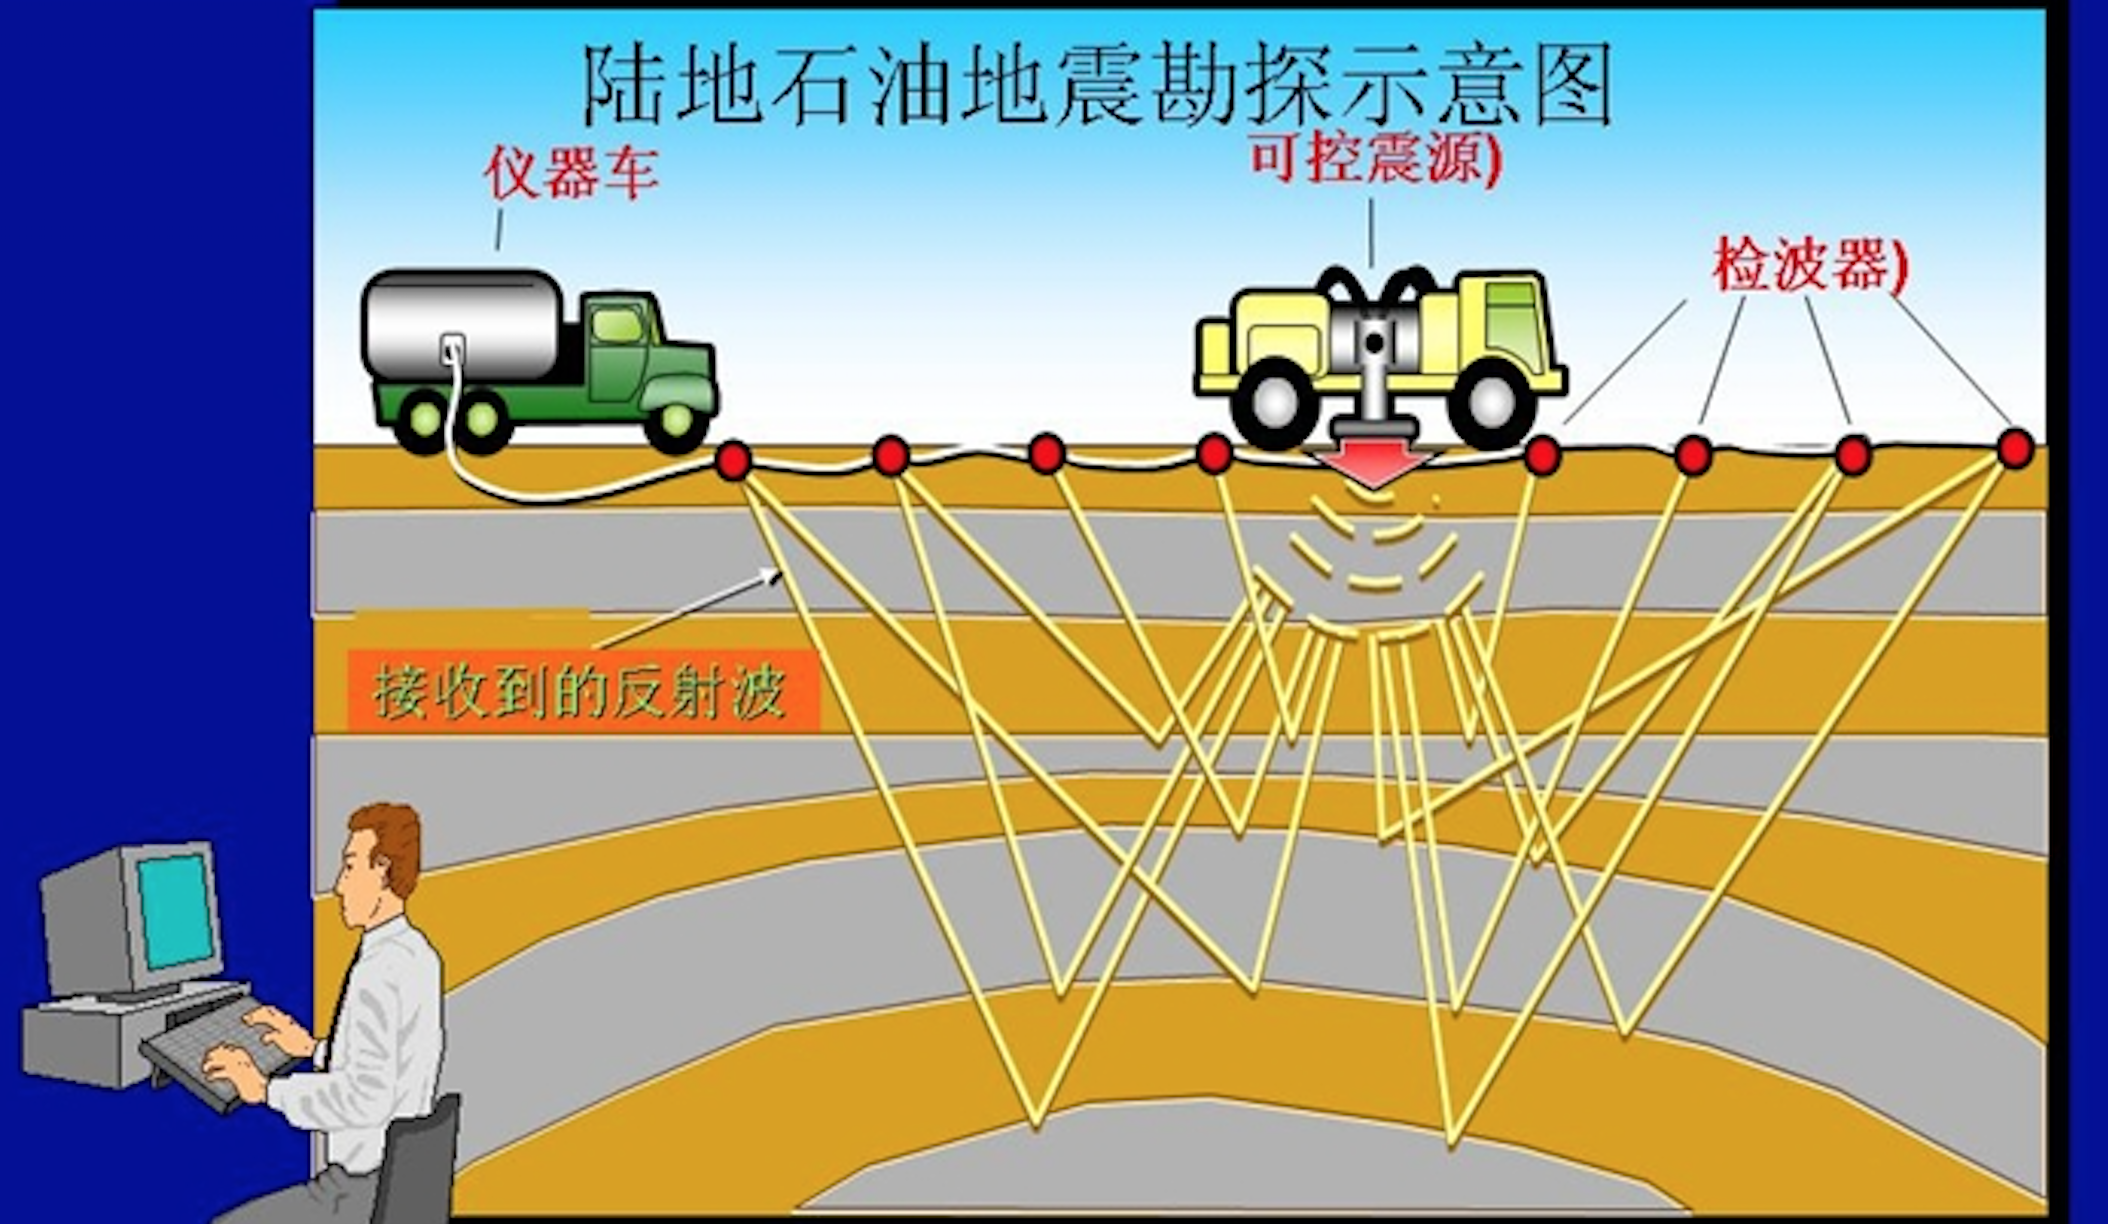
\includegraphics[width=\textwidth]{./Img/seismic2}
	\caption{地震波勘探模型.} \label{figure_seismic}
\end{figure}


由于反问题是高度线性不适定问题 \cite{hadamard1923lectures}, 换言之, 如果我们测量到的数据不准确或是有一个微小的扰动, 都会可能导致相对应的障碍物带来巨大的误差. 因此对反问题做适当形式的转化, 是求解反问题的重要方法. 类似于声波、电磁波, 弹性波反散射问题的方法主要也分为迭代法和直接成像法两种.  

迭代法是一种优化手段, 具体是将观察数据与初值参数构成目标函数, 然后将目标函数最小化的过程.  抽象为如下表达式:
\ben
\min_{\mathbf{m}} \ dist(\mathbf{d}^{obs},\mathbf{{L}}\mathbf{m}),
\een
其中 $\mathbf m$ 表示障碍物边界参数或是非均匀介质参数, $\mathbf{d}^{obs}$ 表示观测数据, $\mathbf{{L}}$ 表示弹性波方程的解算子, $dist(\cdot,\cdot)$ 表示某种距离. 
对于全空间弹性波障碍物散射问题, Li \cite{li2016inverse} 和 Bao \cite{bao2018direct} 提出了利用多频散射数据,基于区域导数的牛顿迭代法.  针对半空间非均匀弹性介质, Mora等人 \cite{mora1987nonlinear,feng2017elastic,elita2018elastic} 提出了最小二乘法反演介质参数的方法.  这些数值迭代方法的优势就是可以定量得到障碍物的边界或是介质参数信息, 但是要求一定的先验信息, 例如边界条件等.  由于每一次迭代都需要解一次弹性波正问题, 这无疑是相当巨大的计算量.  此外,这类优化问题一般都是非凸的, 这导致初值的选择, 迭代收敛性的证明都是比较困难的问题.  

直接成像法的基本思想是构造一个指示性成像函数,代入观测数据后, 该函数值在远离障碍物边界时逐渐衰减; 在靠近边界时, 函数值趋于峰值. 针对二维全空间弹性波反障碍物散射问题, Arens \cite{arens2001linear} 将线性采样法 (Linear Sampling Method) 从声波情形推广了到了弹性波情形.   Alves 和 Kress \cite{alves2002far}, Arens \cite{arens2001linear}, Charalambopoulos \cite{charalambopoulos2006factorization}, 以及  Hu, Kirsch \cite{hu2012some} 等发展了弹性波情形下的分解法 (Factorization Method) .  Ji 等 \cite{ji2018direct} 基于分解法提出了直接成像法,并证明了该函数在障碍物边界上有下界.  然而, 无论是线性采样法还是分解法, 至今都不能应用于弹性波反散射问题的近场数据. 这是因为, 我们没有办法将接收到的近场混合波数据分解成 p 波和 s 波, 除非我们能得到接收点附近领域内的所有数据.  Guzina 等
人 \cite{gintides2012identification} 利用拓扑导数方法对弹性波非均匀介质逆散射问题进行重构.  Chen 和 Huang \cite{ela_reverse} 针对全空间弹性介质扩展障碍物成像问题, 提出了单频加权弹性波逆时偏移方法,并且给出了弹性波逆时偏移方法的分辨率分析,该理论结果表明成像函数均为正值,从而保证了算法的稳定性. 

目前,在数学物理领域中, 对弹性波反散射问题的讨论主要集中于上述的全空间反障碍物散射问题,以及粗糙曲面反散射问题\cite{hu2016factorization,li2016near,liu2019near,hu2018direct},据本文作者所知,至今还极少有数学方面的文献来讨论半空间障碍物模型的.  然而,在地球物理领域中, 地震波勘探就是一个典型的半空间弹性波反散射模型.  因此, 本文将联系实际模型, 基于逆时偏移算法提出半空间弹性波反散射问题的直接成像法. 



\section{逆时偏移方法简介}

逆时偏移 (Reverse Time Migration) 是源于勘探地球物理领域的一种叠前深度偏移方法.  在逆时偏移流行之前, 单程波方程偏移法\cite{claerbout1972downward,gazdag1978wave} 一直是偏移研究的主要课题. 然而, 为了将波动方程分解成单程的上行波方程和下行波方程,需要引入平方根算子\cite{zhanggq1993,Zhang2007,zhang2018itoin}.  该平方根算子是一个拟微分算子,在数值计算时, 数值计算时需要用一系列的积分、微分算子来逼近,这给单程波方程的计算带来非常大的困难. 于是,基于全波方程的逆时偏移法在 1983年被 Whitmore \cite{whitmore1983iterative}, Baysal \cite{baysal1983reverse} 和 Mcmechan  \cite{mcmechan1983migration} 先后提出.  早期, 由于计算资源的匮乏, 工程师们把接收到的弹性波数据利用声波方程来进行逆时偏移 \cite{zhang2009,Zhang08,bleistein2013mathematics,claerbout1985imaging,berkhout2012seismic},但是由于弹性波是包含两种不同波数的 s 波和 p 波的耦合波, 两种波携带着不同的位移信息\cite{yan2008isotropic}.  因此, 发展利用弹性波全波方程的逆时偏移方法是必然的. Chang 和 McMechan \cite{chang1986reverse} 利用弹性波方程将接收到的弹性波数据时逆地外推到地表下, 然后提出了激励时间成像条件 (Excitation time), 而 Hokstad\cite{hokstad1998elastic} 利用 {Lam\'{e}} 势方法作为成像条件.  总之, 这两种成像条件都是互相关成像条件的特殊情形\cite{yan2008isotropic}. 此外, 由于弹性波包含 s 波和 p 波,地球物理学家发展出了两种基于 Helmholz 分解的逆时偏移算法 \cite{yan2008isotropic,sun2001scalar,denli2008elastic,chung2012implementation}.  

第一种方法是将接收到的弹性波数据,反传到接收面附近的浅层区域, 利用 Helmholtz 分解将耦合波场分解成 s 波向量势和 p 波标量势 \cite{etgen1988prestacked,zhe1997prestack}. 随后, 利用相应的 s 波波数与 p 波波数的声波方程将分解后的波正传回接收面. 最后利用传统的声波逆时偏移算法, 对分解完的数据分别进行相应波数的声波反传,随之与相应波数的声波点源互相关成像. 

第二种方法是先用弹性波全波方程将在表面接收到的位移数据反传到地下,然后将反传后的弹性波与点源发出的弹性波都进行波场分解, 最后对分解后的入射波与反传波作互相关\cite{dellinger1990wave}. 
 
总之, 逆时偏移算法的基本大致可以分成两步,第一步是将接收到的波数据作为在接收面上的 Dirichlet 边界条件,而后时逆地反传到背景介质中, 第二步是将入射波和反射波作互相关得出成像函数. 我们在此强调,本文中我们研究的逆时偏移算法不使用波场分解, 而是直接利用接收到的耦合的混合波场数据,经过反传后直接与入射波做互相关.  特别地, 我们的成像函数为 (详见 (\ref{cor2}) ):
\ben
\hat{I}_d(z)=\Im\sum_{q=e_1,e_2}\int_{\Gamma_0^d}\int_{\Gamma_0^d}\,
[\T_D(x_s,z)^Tq][\T_D(x_r,z)^T\overline{u^s_q(x_r,x_s)}]\,ds(x_r)ds(x_s).
\een
这里 $\Ga_0^d=\{x\in\Ga_0: x_1\in (-d,d)\}$, $d>0$, 是半空间表面接收数据的区间, $\T_D(x,z)$ 是 Dirichlet Green 函数在 $\Ga_0$ 上 $e_2$ 方向的应力张量 (详见 (\ref{DGT2}) ). 


关于逆时偏移方法的数学理论分析, 最早是由 Beylkin \cite{beylkin1984inversion,beylkin1985imaging,beylkin1990linearized} 基于广义 Radon 变换, 采用高
频渐近假设或者几何光学近似给出的渐近分析.  但是, 在实际的工程情况下, 这些假设的条件一般都不能满足. 近几年来, Chen 等\cite{chen2013reverse_acou,chen2013reverse_elec,thesis_guanghui} 针对全空间中声波和电磁波反障碍物散射问题, 研究了相应的单频逆时偏移方法来重构障碍物.  他们基于  Helmholtz-Kirchhoff 等式, 在不需要高频假设或几何光学近似的前提下,对算法的分辨率做出了严格分析, 并证明了该成像函数恒为正函数, 从而保证了该数值方法的稳定性. 在文献 \cite{chen2015reverse_planar} 中, Chen 等针对平行平板声波波导反散射问题,提出了基于逆时偏移算法的直接成像法. 在该文章中, 作者提出了广义的 Helmholtz-Kirchhoff 等式,并由此给出了成像分辨率的理论结果. 进一步, 文献\cite{RTMhalf_aco}中作者考虑声波半空间反散射问题的逆时偏移方法,并提出了全新的点扩散函数, 并且给出了分辨率的理论分析.  特别地, 该文章中给出了孔径选取的标准, 以及说明了半空间情形下只能对障碍物面向接收面的那部分进行成像, 这给本文的研究做了很好的铺垫. 

由于在实际的工程应用中, 获取观测数据的强度或振幅 (无相位数据) 比获取该观测数据的相位信息要容易很多. 由此, Chen等 \cite{chen2017phaseless,chen2016direct,chen2017direct,thesis_shaofeng} 基于逆时偏移算法,针对全空间声波,电磁波以及半空间声波反散射问题, 提出了无相位成像算法.  此外, 当障碍物远离发射面和接收面时, 证明了该无相位成像算法与原本的逆时偏移成像方法近似等价,并且给出了相应的误差分析. 




\section{本文内容安排}

本论文安排如下:

第二章中我们将介绍一些后文会涉及的函数空间,并且叙述后文会用到的经典的数学定理. 

第三章中我们利用 Fourier 变换推导出 Neumann Green 函数和 Dirichlet Green 函数, 并且研究 Green 函数的相关性质.  而后,通过极限吸收原理研究半空间弹性波散射问题解的适定性. 

第四章中我们首先介绍针对点源成像的点扩散函数, 然后提出重构半空间扩展障碍物的基于弹性波逆时偏移方法的直接成像法, 最后利用点扩散函数和散射系数逼近给出了该障碍物重构算法的分辨率分析. 

第五章中我们针对本论文中的研究进行总结, 并且叙述相关可待研究的问题. 

